\vspace{-.15in}\section{Research Plan and Methodology}
\label{sec:plan}

% \vspace{-.075in}
% 
% % \xxx strengthens the reliability of datacenter 
% % computing with a holistic methodology.
% This section first proposes the three objectives in this proposal.
% The first two objectives include preliminary results. 

\vspace{-.15in}\subsection{Objective 1: 
preventing big-data computation leakage with \kakute}\label{sec:obj1}
\vspace{-.075in}
% % 
This section presents major challenges in existing DFT systems 
(\S\ref{sec:ift-problem}) and \kakute (\S\ref{sec:kakute}).

\vspace{-.15in}
\subsubsection{Challenges: existing DFT systems are too slow and incomplete for 
big-data} 
\label{sec:ift-problem}\vspace{-.075in}

Although DFT is a powerful access control technique, existing DFT systems incur 
high performance overhead, especially for data-intensive computations. For 
instance, we ran a recent DFT system Phosphor~\cite{oo14:phosphor} in Spark 
with a WordCount algorithm on a small dataset of merely 200MB, and we observed 
128X longer computation time compared with the native Spark 
execution~\cite{kakute:acsac17}. The second challenge is completeness: 
big-data frameworks usually contain \emph{shuffle} operations, which 
redistribute data and results across computers. However, most existing DFT 
systems ignore data flows across computers. For the 
few~\cite{cloudfence:raid13} who support cross-host data flows, transferring 
all tags in shuffles consumes excessive network bandwidth.
% Therefore, efficient 
% cross-host tag propagation is crucial but missing in DISC.

\vspace{-.15in}\subsubsection{\kakute: a fast, precise DFT system for big-data} 
\label{sec:kakute}\vspace{-.075in}

\begin{figure}[h]
    \centering
    \begin{minipage}{.48\textwidth}    
          \vspace{-.1in}
        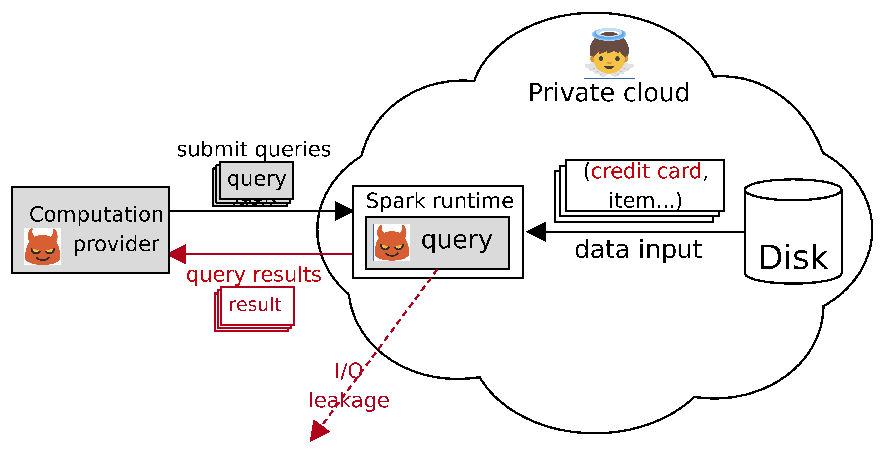
\includegraphics[width=0.95\textwidth]{figures/threat_private.ps}
         \vspace{-.1in}         
        \caption{Threat model of \kakute. Red colors means sensitive data or 
leaking channels. Shaded (grey) components may leak data, and \kakute is 
designed to defend against them.}
        \label{fig:falcon-arch}
    \end{minipage}
    \hspace{.1in}
    \centering
    \begin{minipage}{0.48\textwidth}
         \vspace{-.1in}
        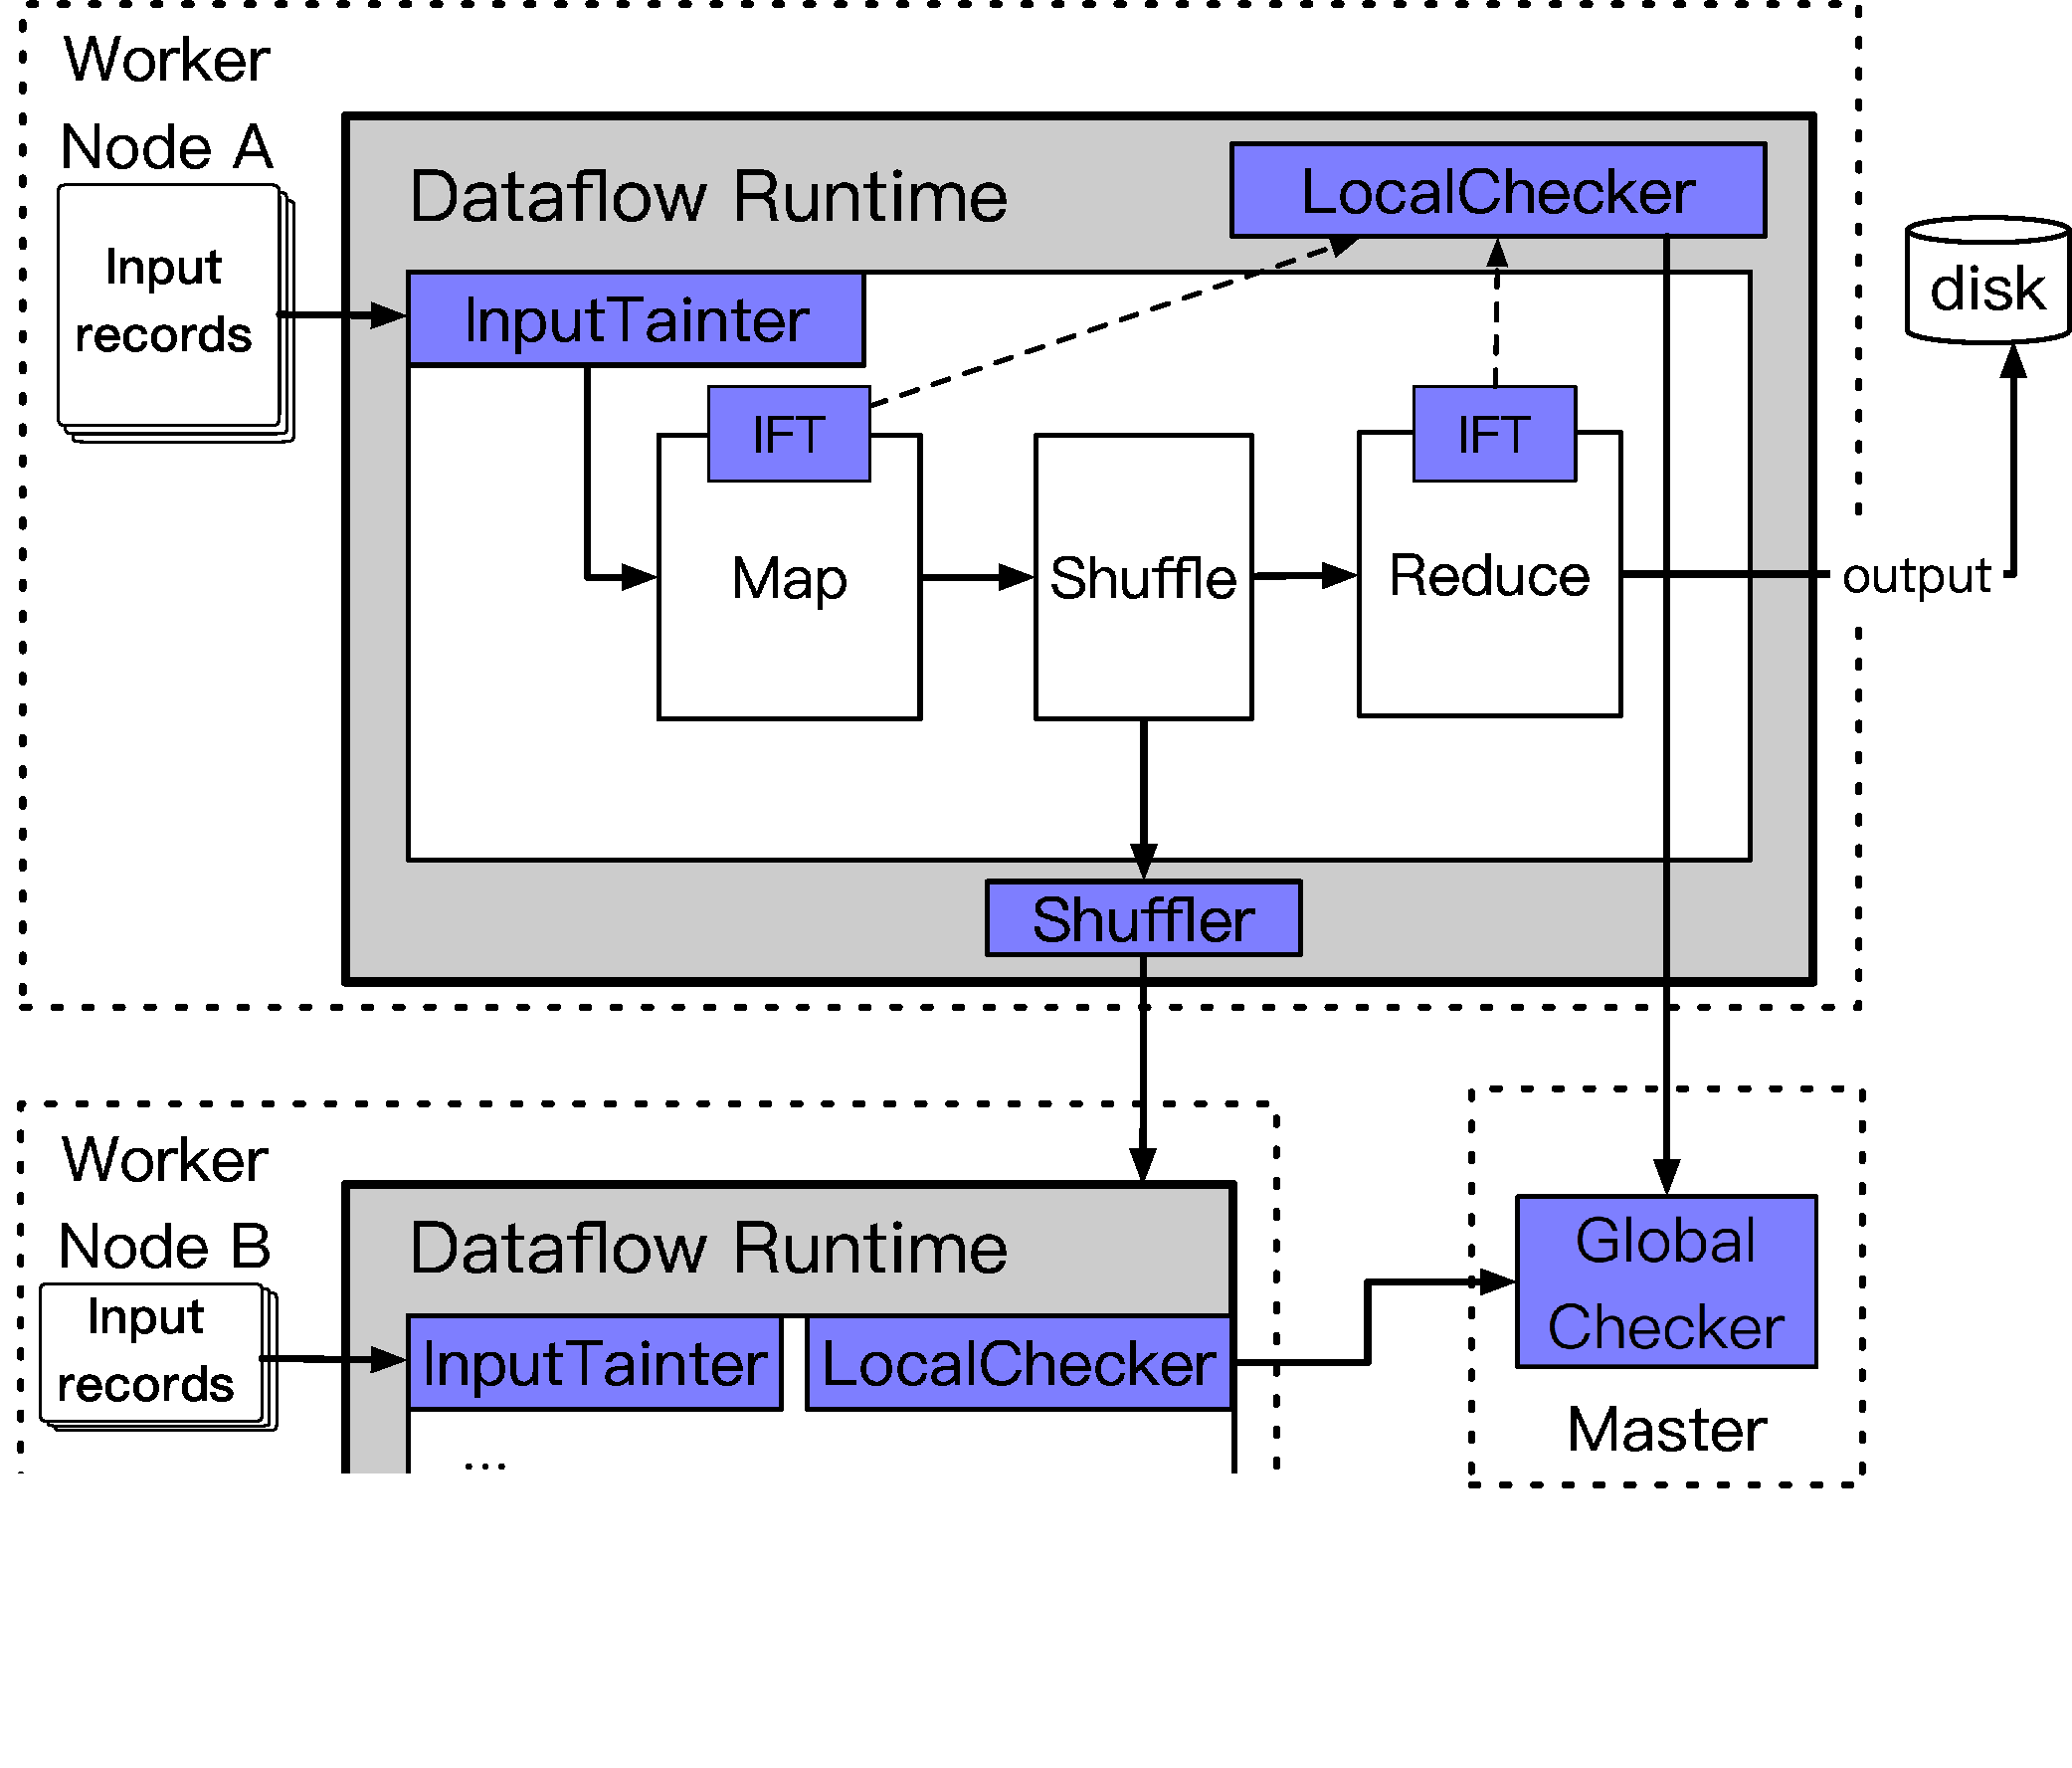
\includegraphics[width=0.95\textwidth]{figures/kakute_arch.ps}
         \vspace{-.4in}
        \caption{\kakute architecture. \kakute's key components are shaded 
(and in blue).}
        \label{fig:falcon-protocol}
    \end{minipage}
\end{figure}

We present \kakute, the first precise and complete DFT system for big-data 
frameworks. Our key insight to address the DFT performance challenge is that 
multiple fields of a record often have the same tags with the same sensitivity 
level. For example, in an Taobao order record $\langle$\vv{time}, 
\vv{userId}, \vv{productID}$\rangle$, only the \vv{userId} field is 
sensitive, while the other fields are insensitive and they can share the same 
tag. Leveraging this insight, we present two new techniques, \lazyp and 
\tagcache. \lazyp avoids unnecessary tag combinations by only keeping the 
\textit{lineage of tags} in the same self-defined queries, while \tagcache 
reduces memory usage by sharing tags among multiple fields in each record. To 
tackle the completeness challenge, \kakute completely captures inter-computer 
data flows (shuffles), and it efficiently reduces the amount of 
transferred DFT tags using \tagcache. Both techniques are illustrated in 
Appendix (c) of this proposal.

Figure~\ref{fig:falcon-arch} defines \kakute's threat 
model. Figure~\ref{fig:falcon-protocol} shows \kakute's design. The 
InputTainter component provides easy-to-use APIs for data providers to 
automatically tag sensitive fields. The DFT component is enabled in 
self-defined functions. The Local- and Global-Checker detect and 
prevent illegal flows of sensitive fields (\eg, credit cards flow to IO 
functions in self-defined functions). Shuffle operations across computers are 
intercepted and tags are added. Therefore, DFT is completely captured across 
computers.

We will implement \kakute and integrate it with Spark. We will leverage 
Phosphor~\cite{oo14:phosphor}, an efficient DFT system working in the Java 
byte-code level. \kakute instruments computations of a Spark worker process
to capture data flows inside self-defined-functions. \kakute provides different 
granularities of tracking with two types of tags: \func{Integer}
and \func{Object} tags. \func{Integer} provides 32 distinct tags for 
identifying 32 sensitivity levels, suitable for detecting data leakage and 
performance bugs. \func{Object} provides an arbitrary number of tags, which is 
suitable for data provenance and programming debugging.
% \kakute provides a 
% unified API to tackle diverse problems.
% Based on this unified API, we 
% will implement 4 built-in checkers for \appsn security and reliability 
% problems: sensitive information leakage, data provenance, programming and 
% performance bugs. 

\begin{wrapfigure}{r}{7cm}
  \vspace{-.1in}
  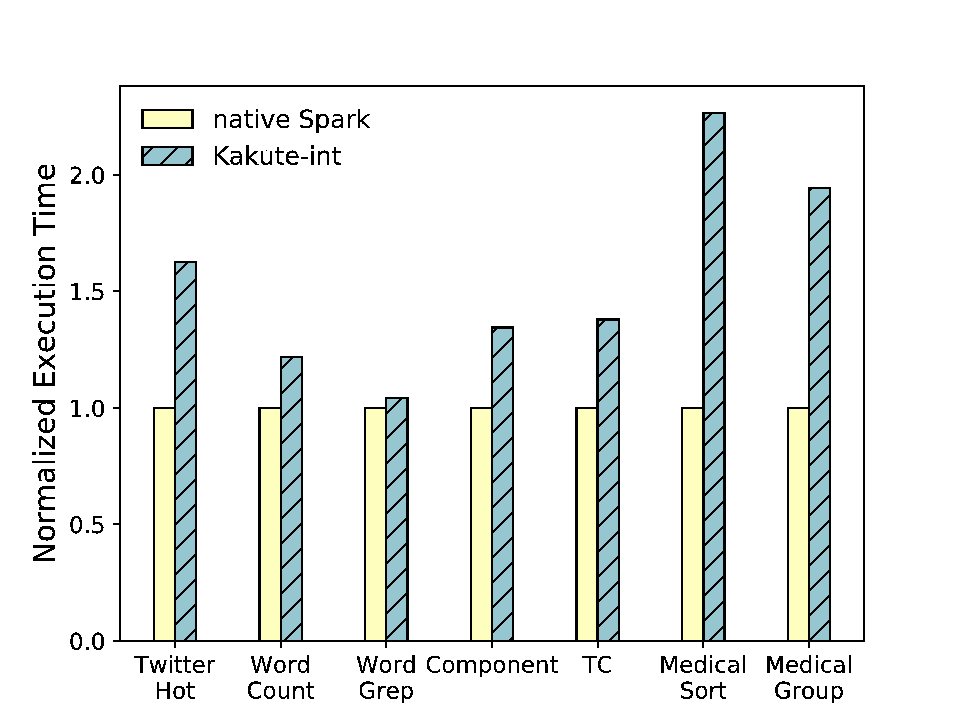
\includegraphics[width=7cm]{figures/time_overhead.ps}\\
  \vspace{-.3in}
  \caption{\kakute execution time normalized to native Spark executions. 100\% 
means no overhead.}
  \label{fig:scalability}
\end{wrapfigure}

\para{Preliminary results.} We have implemented a \kakute prototype 
and evaluated it on \appeval popular big-data algorithms, including three text 
processing algorithms WordCount~\cite{spark:example}, 
WordGrep~\cite{newt:socc13} and TwitterHot~\cite{spark:example}, two graph 
algorithms TentativeClosure~\cite{spark:example}
and ConnectComponent~\cite{spark:example}, and one analysis program 
MedicalGroup~\cite{pigmix}.
We evaluated these algorithms with 
real-world datasets that are comparable with related 
systems~\cite{vldb16:output, icse16:bigdebug, vldb15:titian}.
Our evaluation shows that: (1) \kakute 
incurred merely \timeavg overhead (Figure~\ref{fig:scalability}) with 
\func{Integer} tag, about two orders of magnitudes faster than a recent DFT 
system Phorspor~\cite{oo14:phosphor}; and (2) \kakute effectively 
detected 13 real-world security and performance bugs presented in other 
papers~\cite{arthur:dave2013,icse16:bigdebug,airavat:nsdi10}. These promising 
preliminary results have been presented in ACSAC '17 and TPDS '17.

% In \xxx, all replicas directly write to destination
% replicas' memory and poll messages from local memory to receive messages, and 
% our runtime system handles other technical challenges such as checking message 
% delivery and recovering replica failures.











% \begin{figure}[!htb]
% \centering
% 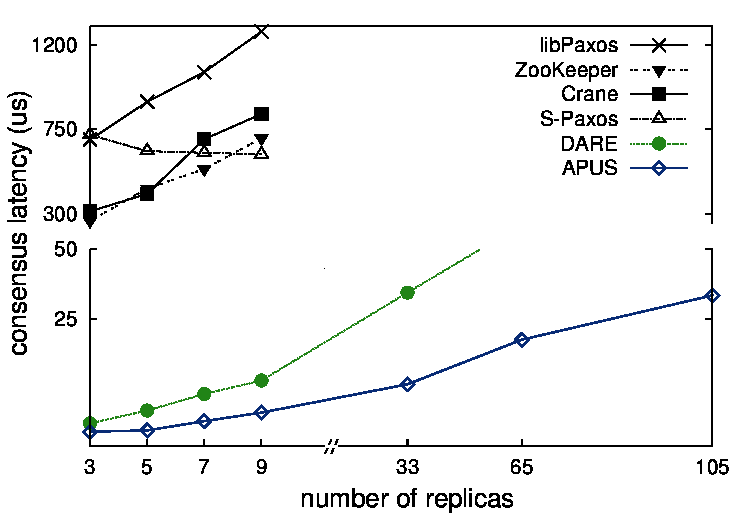
\includegraphics[width=0.25\textheight]{figures/traditional_paxos_latency.ps}
%         \vspace{-.2in}
%         \caption{Consensus latency of six \paxos protocols. \falcon is fastest 
% and scales the best.}
%         \label{fig:scalability}
% \end{figure}


% When changing the replica group size 
% from 3 to 105 (a 35x increase), \falcon's consensus latency increases merely 
% from \xxxlatencythree \us to \xxxlatencyonezerofive \us (a \xxxscalability, 
% sub-linear increase).
% Crane. Falcon. Say Crane is first version. Falcon 
% totally subsumes Crane. Falcon also has initial results.


% ~\cite{pig:vldb08}
% ~\cite{hadoop}
\para{Future directions.} We will extend \kakute in 
three directions. First, we will port \kakute onto more big-data frameworks, 
including \pig~\cite{pig:vldb08} and \hadoop~\cite{hadoop}. Second, we will 
extend \kakute to detect broader types of real-world security bugs. Third, we 
will apply \kakute to augment other complementary privacy techniques, including 
anonymization techniques and differential privacy (\textbf{Objective 2}). 

\vspace{-.15in}\subsection{Objective 2: developing the Fine-grained 
Differential Privacy (FDP) technique}\label{sec:obj2}\vspace{-.075in}



\kakute (\textbf{Objective 1}) strictly prevents
sensitive data flowing to IO functions or query results, but in some scenarios 
it is still desirable to let computation providers acquire aggregation 
results (\eg, the sum of citizens who have got cancer in a country) 
on sensitive fields as long as individual information is not leaked. 
Differential privacy~\cite{Dwork2006Differential} can enforce statistical 
bounds on 
aggregation results and prevent individual information leakage, so it is 
complementary to DFT and has attracted much attention recently.

% Differential privacy is a robust privacy standard proposed by Dwork et
% al.
% His work shows that differential privacy can be achieved by adding
% Laplace distributed noise whose scale is related to the sensitivity of queries.
% This simple algorithm can handle all kinds of queries but inevitably has some
% drawbacks. For instance, the number of query is limited and too much noise will
% be injected to continuous queries. To reduce noise magnitude, a 
% sample-and-aggregation
% framework~\cite{differentialdp:stoc11} is proposed.

\vspace{-.15in}
\subsubsection{Challenge: existing differential privacy techniques are 
coarse-grained and thus inaccurate} 
\label{sec:ift-problem}\vspace{-.075in}

Existing differential privacy techniques often suffer from low accuracy for 
query results. To prevent computation providers revealing individual 
data, differential privacy typically adds noise either on input data 
records or query results. However, due to the lack of precisely tracking 
how inputs are computed and propagated to outputs, to enforce statistical 
guarantee on outputs, differential privacy often conservatively add the same 
noise to all fields of a data record and to all records, causing inaccurate 
results. For instance, prior work~\cite{differentialresult:vldb15} reports 
more than 30\% loss of accuracy when the security guarantee is high (the 
probability of leakage is low). Therefore, a KMeans program will return 
centroids far from the accurate ones. This low accuracy makes results useless as 
it is much larger than the KMeans training error rate (a few percents).

\vspace{-.15in}
\subsubsection{FDP and its new algorithm} 
\label{sec:ift-problem}\vspace{-.075in}

\begin{figure}[!htb]
    \begin{minipage}{0.44\textwidth}
%         \vspace{-.1in}
        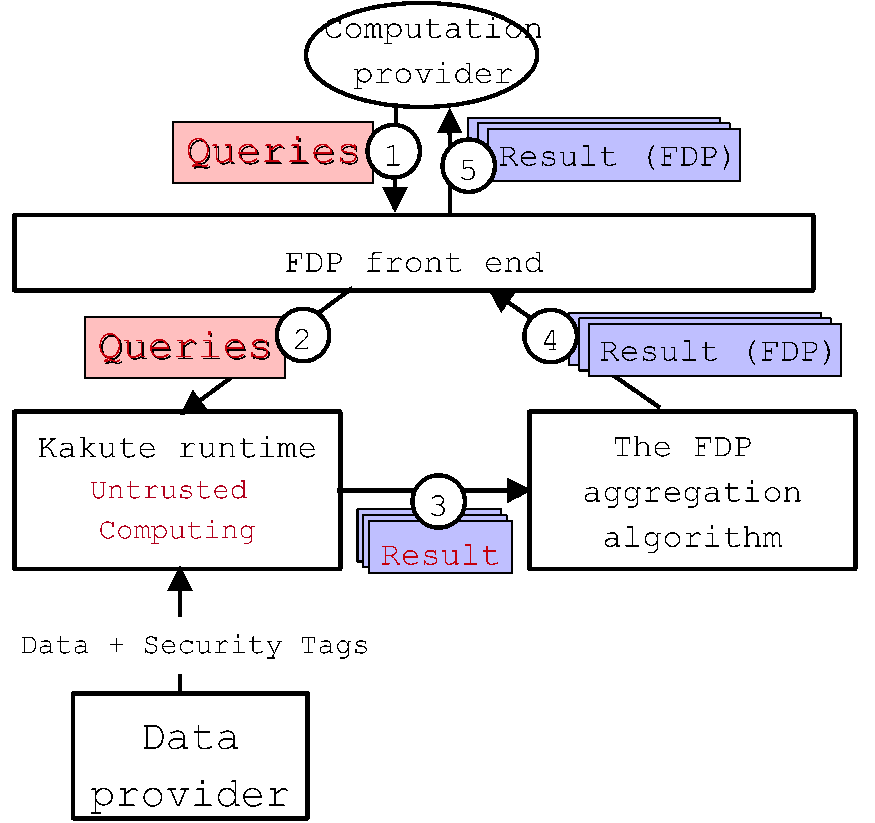
\includegraphics[width=0.3\textheight]{figures/selective_arch.ps}
        \vspace{-.1in}
        \caption{The workflow of FDP with five steps.}
        \label{fig:vm-tree}
    \end{minipage}
    \begin{minipage}{0.54\textwidth}
      \vspace{-.2in}
      \centering

      
      
      \begin{algorithm}[H]
\SetAlgoLined
\KwIn{Dataset T, dataset size N, privacy budget $\varepsilon_k$ for security 
level k,
  output range (min, max)}
  n = a suitable partition

 \For{$i\leftarrow 1$ \KwTo $n$}{
    $O_i$ $\leftarrow$ $f(T_i)$\;
    if $O_i$ $>$ max, $O_i$ $\leftarrow$ max
    if $O_i$ $<$ min, $O_i$ $\leftarrow$ min
 }
 \For{dimension $j$ of the output $O$}{
    k $\leftarrow$ $getTagLevel(O_{j})$\;
    $O_j$ $\leftarrow$ $\dfrac{1}{n}\sum\limits_{i=1}^n O_{ij} + Lap(\dfrac{max 
- min}{n\varepsilon_{k}})$
  }
  \KwOut{$O$}
 \caption{The FDP aggregation algorithm}
 \label{algo:combined}
\end{algorithm}
      
      
      
      
    \vspace{-.1in}
    %     \caption{Sketch of path slicing algorithm}

%         \label{fig:algo}

\end{minipage}
    \vspace{-.1in}
\end{figure}

Our key insight is that DFT and differential privacy can complement each other, 
getting the best of both worlds. Considering each data record, DFT can 
precisely track how sensitive data fields flow to which query result, so 
differential privacy needs only add noise to the sensitive input fields or 
results. Considering all data records, DFT can also distinguish which records 
have higher security sensitivity levels, then we can add more noise accordingly.

This insight nurtures Fine-grained Differential Privacy (FDP). In FDP, each 
record belongs to a user who assigns a security tag to all its data records.
A security tag that is related to the privacy budget $\varepsilon$ (or accuracy 
level). When the privacy budget is high, the probability of leakages is high.
We adopt the personalized differential privacy model in recent
work~\cite{pdp:icde15}. $\Phi(x)$ return the $\varepsilon$ of a particular 
record x. The threat model of FDP is the same as \kakute's 
(Figure~\ref{fig:falcon-arch}), because FDP aims to defend against malicious 
computation providers in private clouds. 

\begin{definition}{Differential Privacy}
For two neighbor dataset $D$ and $D'$ differing at record x,
a mechanism ${\cal M}(y)$ is differentially private with the following 
condition:
\begin{align}
Pr[{\cal M}(D) \in O] \leq e^{\Phi(x)} \times Pr[{\cal M}(D') \in O]
\end{align}
\end{definition}

Intuitively, Differential Privacy guarantees that the probability of
producing different result with neighboring dataset is low. For the 
personalized model, the probability is different for records belonging to 
different users, so that different users have various levels of protections.

To start with, we need to determine the relation of the privacy budget and the 
security level (a \vv{getTagLevel} function). We adopt a deterministic model, 
and there are 6 security levels: insecure, $dp_1$, $dp_2$, $dp_3$, $dp_4$ and 
non-released. Insecure records can be release directly, while non-released can 
not be used in any computation to the final result. $dp_1$ to $dp_4$ varies in 
terms of their privacy budgets for differential privacy.
% We may also consider the $(\delta, \varepsilon)$-differential privacy model.

% We extend the differential privacy model developed in previous
% work~\cite{differentialdp:stoc11}. We introduce two noise calibration model
% that make use the fact that different record may have
% different security level (protection level).


\begin{theorem}{Laplace Mechanism~\cite{Dwork2006Differential}}
  Adding noise with Laplace distribution $Laplace(\dfrac{\Delta 
f}{\varepsilon})$ enforces
  Differential Privacy, and global sensitivity $\Delta f$ is defined as
  \vspace{-.1in}
  \begin{align}
    \Delta f = max || f(D) - f(D') ||_1
  \end{align}
\end{theorem}

To enforce differential privacy, one approach is to use the $\varepsilon$ 
inferred by the highest security level of each dimension and to add noise to 
the output directly, but this approach is too naive for the diversity of 
security levels. Instead, we adopt the sample-and-aggregate approach in 
previous work~\cite{differentialdp:stoc11}. In this approach, data is 
partitioned into multiple parts (each part has a size of $m$). Each partition 
can have different sensitivity levels. The aggregator adds noise to the 
result of each partition according to its security level. Data 
is partitioned into multiple parts denoted as $p_1$, ..., $p_n$.
The security level and its corresponding $\varepsilon$ are $\varepsilon_1$,
..., $\varepsilon_n$.

\begin{theorem}
  For any output record in $O$, the
  estimator is $max_{i \le k}(\varepsilon_i)$-differentially private.
\end{theorem}
\begin{proof}
  For each dimension, we can divide the output dataset $D$ as k disjoin parts 
$D_1$, $D_2$,
  ..., $D_k$ according to their security levels. According to 
prior work\cite{pointestimation:smith08},
  each $f(D_i)(i \le k)$ is $\varepsilon_k$-differentially private.
  For each $D_i$, we have $Pr[f(D_i) \in S] \le e^{\varepsilon_i}Pr[f(D'_i) \in 
S]$, suppose $\varepsilon_{max} = max_{i \le k}(\varepsilon_i)$, \\
  \vspace{-0.1in}
  \begin{equation} \label{eq1}
  \begin{split}
  Pr[f(D)] & = Pr[f(D_1 + D_2 + \ldots + D_k)] \\
   & = e^{\varepsilon_1}Pr[f(D'_1)] + \ldots + e^{\varepsilon_k}Pr[f(D'_k)] \\
   & \le  e^{\varepsilon_{max}}(Pr[f(D'_1) + \ldots + Pr[f(D'_k)]]) \\
   & = e^{\varepsilon_{max}}Pr[f(D')]
  \end{split}
  \end{equation}
  Therefore, $f(D)$ is $max_{i \le k}(\varepsilon_i)$-differentially private.
\end{proof}

In the above aggregation algorithm, the error of the final result comes from 
two parts: the Laplace noise error and the partition error. It is crucial to 
reduce the final error incurred by this algorithm while keeping the 
differential security guarantee. We can adopt a hill-climbing approach (future 
work).

\para{Future directions}. We will fully develop this FDP technique by going 
along three directions. First, we will continue to optimize the algorithm and 
reduce its final error rate. Second, we will do an extensive study on 
real-world big-data queries and quantify the improvements on result accuracy. 
Third, currently we propose a end-to-end differentially private computation
system, which adopts a personalized differential privacy 
model~\cite{pdp:icde15} and improves usability without reducing the security 
guarantee. In future explorations, we can consider an even more fine-grained 
$(\varepsilon, \delta)$-differentially~\cite{differntialprivacy:tcc06}
private model.


\vspace{-.15in}\subsection{Objective 3: creating a privacy-preserving compiler 
for big-data queries in public clouds}\label{sec:obj3}\vspace{-.075in}

% In order to reduce maintainance costs, more and more sensitive data are stored 
% and processed in public clouds (\eg, Amazon EC2 and Dropbox). Although data can 
% be securely encrypted while in rest, recent real-world privacy breaches have 
% shown that data are often leaked while being processed. The reason is that 
% homomophic encryption is still pre-mature (a notable analytic database 
% CryptoDB~\cite{cryptdb:sosp11} reports a 1000X overhead compared with
% the unencrypted execution), and most data is being processed in plaintext. 

Recent real-world privacy breaches have shown that sensitive data are often 
leaked while being processed in public clouds, including clouds compromises on 
external attacks~\cite{icloud-breach} and 
insider attacks~\cite{top-threats}. Trusted Execution Environment 
(TEE) is a promising technique to protect computation on public clouds even if 
the cloud's operating system is compromised. For example, 
Intel-SGX~\cite{intel-sgx} runs programs in a enclave, so code and data are 
protected and can not be seen by the attackers. Meanwhile, SGX is good fit for 
big-data queries because these queries are data-intensive in userspace and they 
hardly invoke system calls (OS kernel can easily break SGX's security on 
memory). A latest big-data analytic system Opaque~\cite{opaque:nsdi17} reports 
only 30\% overhead compared to native, insecure executions.

\vspace{-.15in}
\subsubsection{Challenges: existing SGX-based systems require rewriting 
queries and have too-large TCB} 
\label{sec:ift-problem}\vspace{-.075in}

Despite recent advances (Opaque~\cite{opaque:nsdi17}, VC3~\cite{vc3:sp15}, 
Azure/Coco~\cite{azure:coco}, and SGX-BigMatrix~\cite{bigmatrix:ccs17}) on 
building SGX-based systems for big-data, two major challenges 
remain. First, enclaves require completely rewriting the readily pervasive Java 
big-data queries into C++~\cite{opaque:nsdi17,vc3:sp15,azure:coco}, a 
time-consuming and error-prone process. 
Second, to easy implementation, existing systems typically run the entire 
language runtime (\eg, JVM or Python runtime~\cite{bigmatrix:ccs17}) within SGX, 
causing the Trusted Computing Base (TCB) to be too large and vulnerable (\eg, 
JVM has millions of lines of code from many companies and is vulnerable to 
insider attacks~\cite{top-threats}).
% SGX-BigMatrix~\cite{bigmatrix:ccs17} proposes a secure and oblivious 
% vectorization
% abstraction for Python, but it needs to rewrite programs with its abstraction.

\vspace{-.15in}
\subsubsection{\maat: a just-in-time (JIT), privacy-preserving Java compiler 
for big-data queries} 
\label{sec:ift-problem}\vspace{-.075in}

\begin{figure}[h]
    \centering
    \begin{minipage}{.4\textwidth}    
          \vspace{-.1in}
        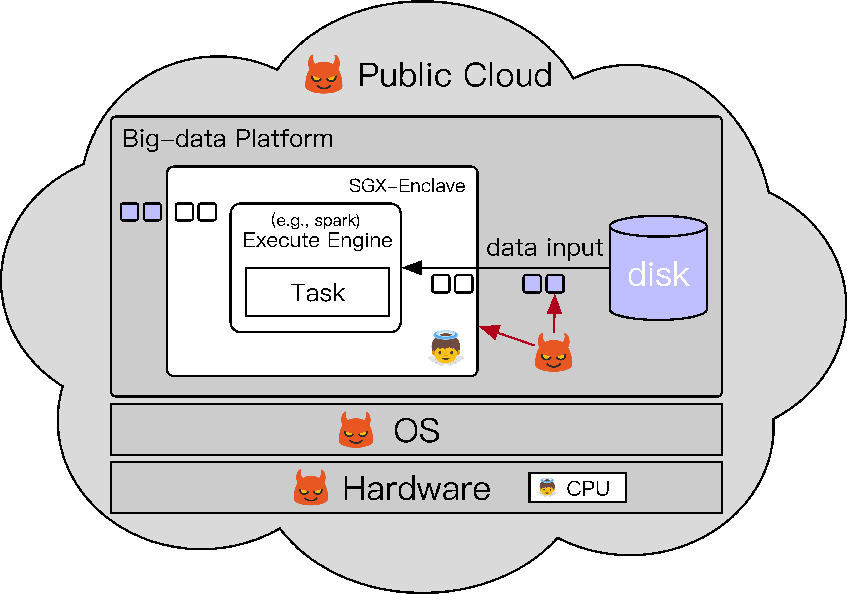
\includegraphics[width=0.95\textwidth]{figures/threat_public.ps}
%          \vspace{-.1in}         
        \caption{Threat model of \maat. Data records with blue color are 
encrypted, and white color are plaintext. Shaded (grey) components may leak 
data, and \maat is designed to defend against them.}
        \label{fig:maat-threat}
    \end{minipage}
    \hspace{.2in} 
    \centering
    \begin{minipage}{0.4\textwidth}
         \vspace{-.1in}
        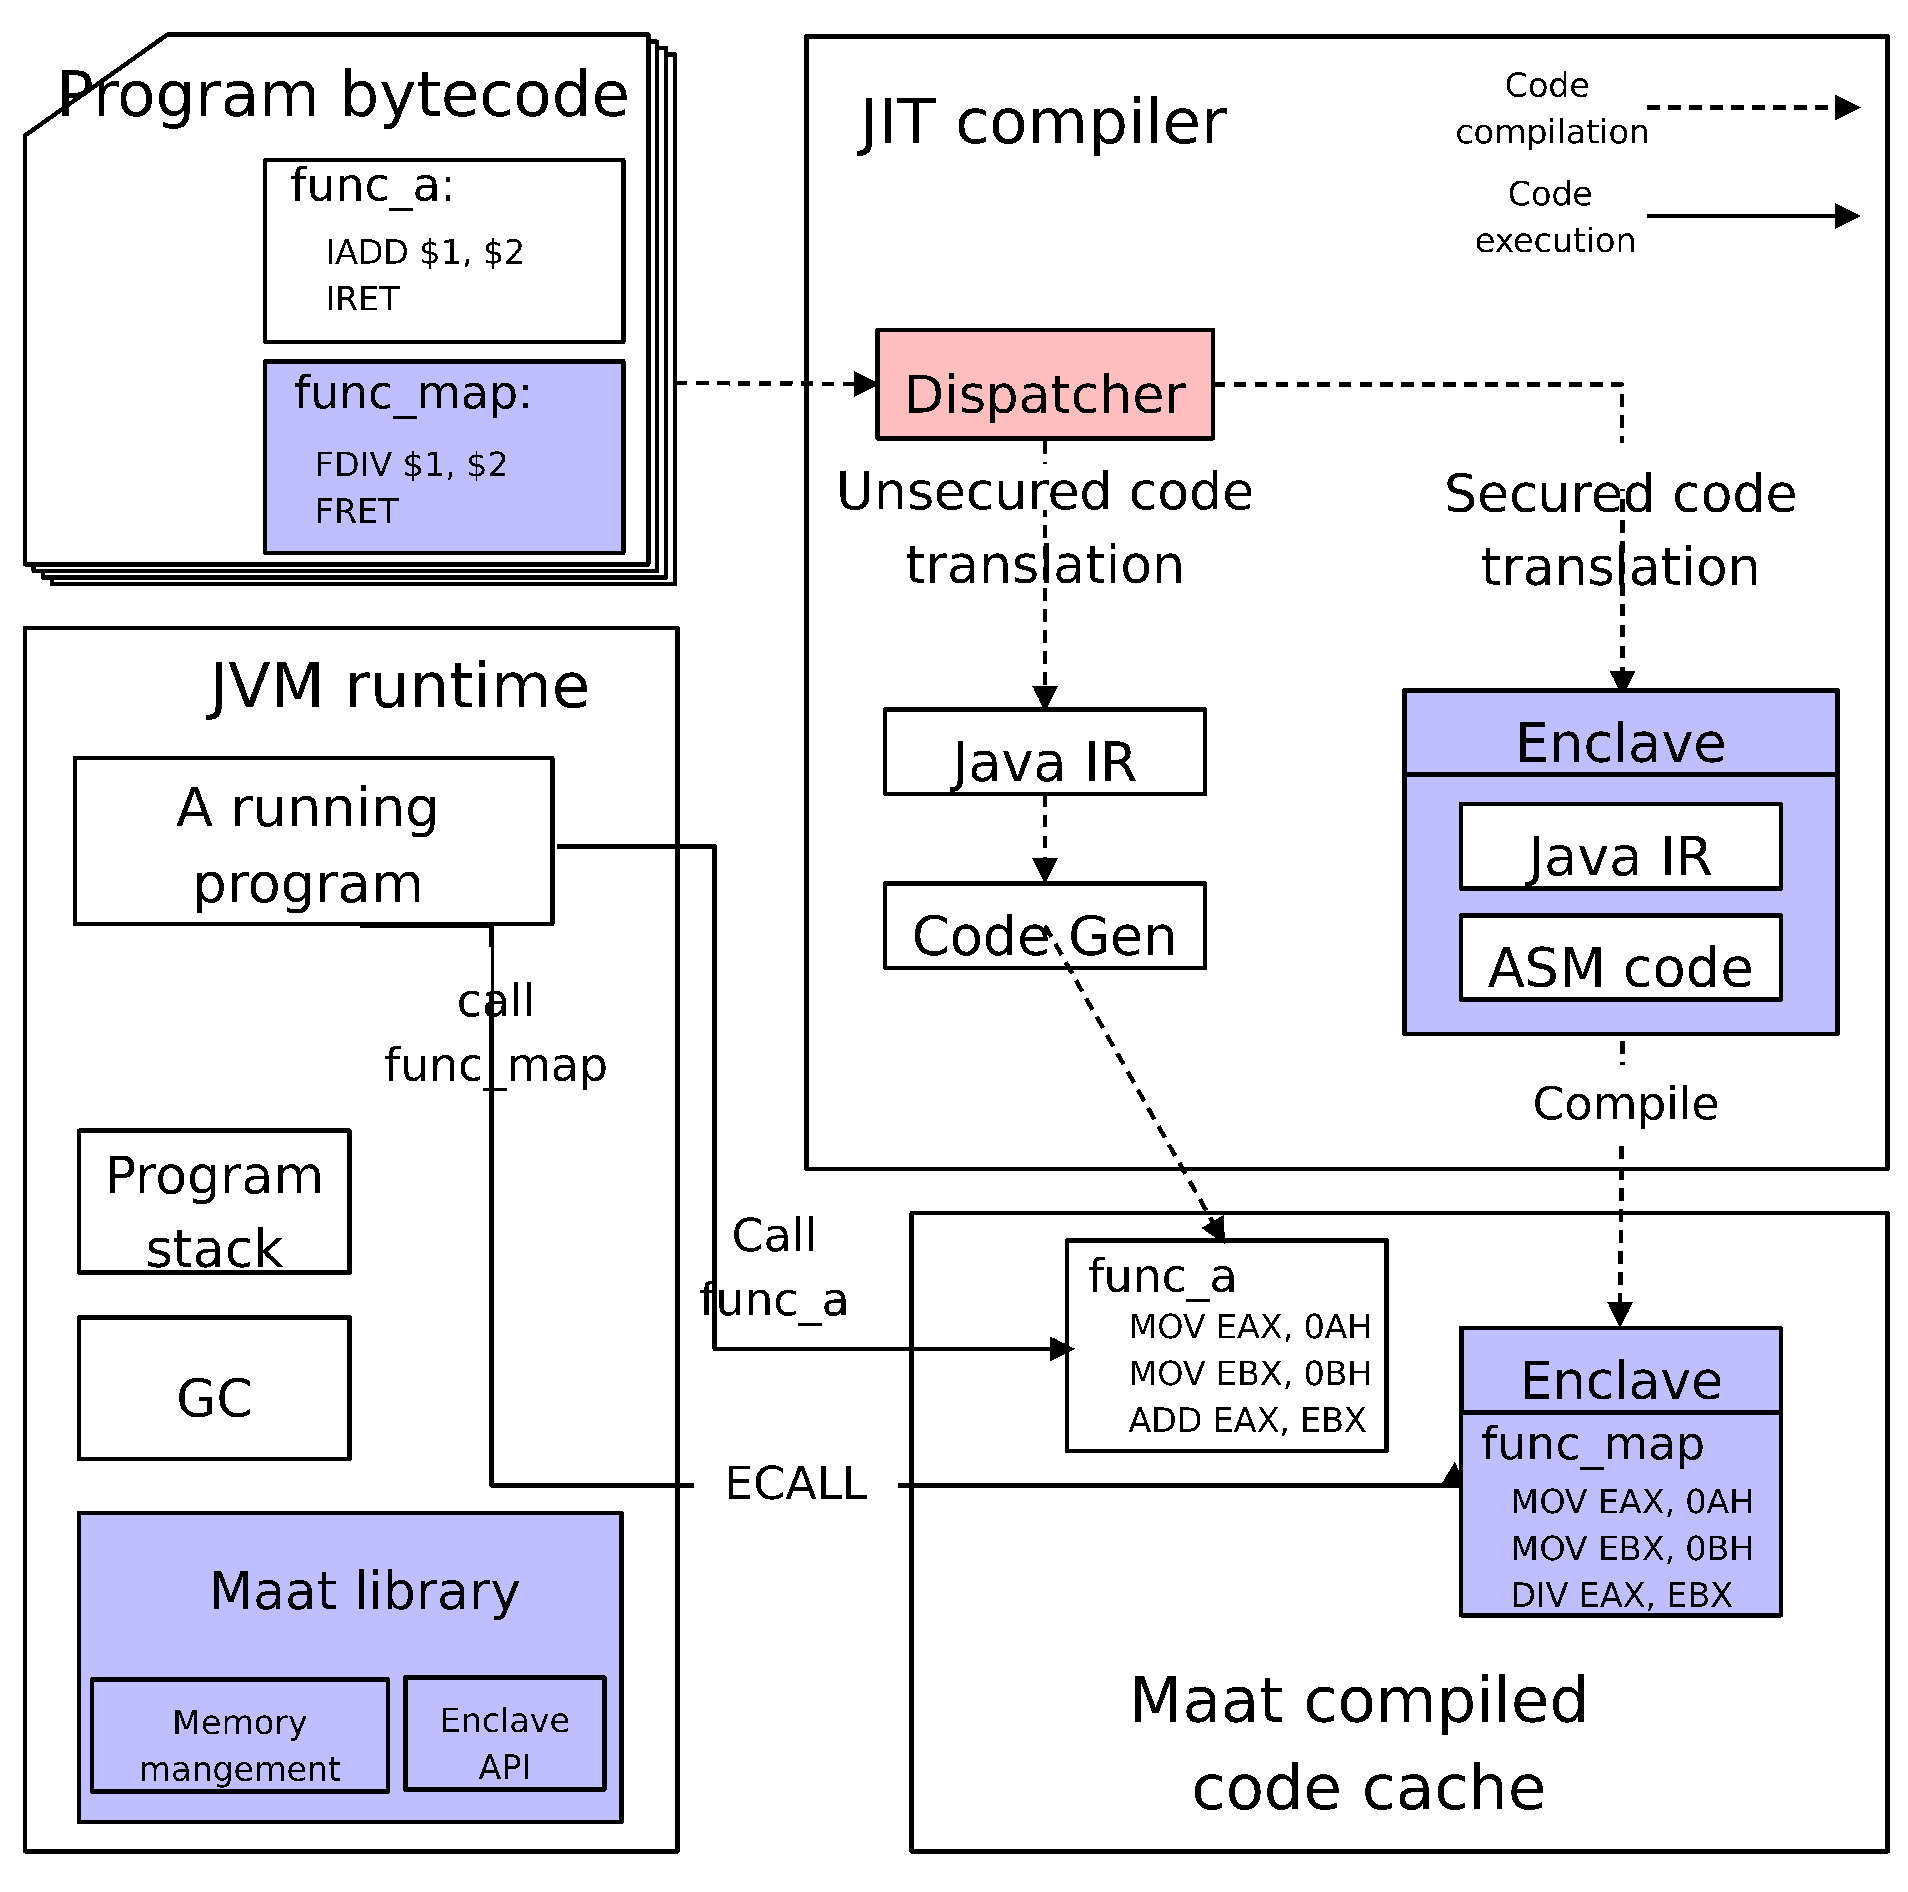
\includegraphics[width=0.95\textwidth]{figures/jit_arch.ps}
         \vspace{-.1in}
        \caption{\maat JIT compiler architecture. Key components are 
shaded (and in blue).}
        \label{fig:maat-arch}
    \end{minipage}
\end{figure}

We propose \maat, the first compiler that runs unmodified Java big-data queries 
in SGX enclaves securely with minimal TCB (\ie, the TCB contains only SGX and 
self-defined code itself). \maat works as a Java JIT compiler which 
automatically compiles self-defined big-data functions (\eg, 
\vv{map}/\vv{reduce}) into SGX-compatible assembly instructions. 
Therefore, the 
JVM itself does not run in \maat's enclaves.

The goal of \maat is to preserve the confidentiality of data while being 
processed in public clouds. Other attacks such as changing execution paths 
(\ie, integrity) have been well defended in prior work~\cite{jitguard:ccs17}, 
and \maat can directly use it.

Figure~\ref{fig:maat-threat} shows \maat's threat model: both SGX and 
computation providers are trusted, and cloud providers are malicious. Figure 
\ref{fig:maat-arch} shows the architecture of \maat. In \maat, both the 
translation of self-defined code and the execution of the code are protected by 
enclaves, so that even if the cloud's OS compromised, it can not see the 
executions of big-data queries or inject malicious code into the queries during 
\maat's translation.
% Self-defined functions and data processed by these 
% functions are protected by \maat . The Java byte-codes of these functions are 
% compiled to enclave-comptabile assembly code.

Our \maat architecture contains two software components: our JIT translator 
and our own management library. The JIT translator is a thin layer which 
translate a Java bytecode instruction into a number of SGX-compatible 
assembly instructions. For instance, in Figure~\ref{fig:maat-arch}, an 
\func{fdiv} Java bytecode instruction translates to two \func{mov} and one 
\func{div} assembly instructions). The memory management library is for our own 
use of encryption/decryption on data records and maintaining SGX memory for the 
queries at runtime. We will proactively implement these two components to be 
easy to verify (use as few as function recursive calls and loops) as in other 
verification practice~\cite{xi:sosp17}, and we plan to use state-of-the-art 
verification techniques~\cite{xi:sosp17} to verify both of them. Then, we do not 
need to include them in \maat's TCB, greatly reducing its TCB.
% Specifically, we plan to implement the two 
% components .


% We don't plan to use OpenJDK as our management library 
% because it contains up to millions lines of code, which is impractical for 
% formal verifications as it is time-consuming with current verification methods 
% (\chref{sec:others-work}).



One subtle performance challenge for \maat is that it should have reasonable 
performance overhead compared to native executions. When calling into and 
out of a function in enclaves, an ECALL and OCALL will be invoked in the CPU 
and enclave transitions are invoked. Such transitions are several hundreds 
times slower than user function calls. Moreover, encryption and decryption on 
data records are invoked during such transitions. Our study on a SGX-based 
big-data system Opaque~\cite{opaque:nsdi17} shows that it incurs 3.4k enclave
transitions for processing only 10k data (with two queries \vv{select} and 
\vv{groupBy}), which confirms the challenge.

% In fact, these processing functions can be pipelined and processed in a single
% enclave function. Our project takes reducing transitions as one of our targets.



% Cost-based Compilation and Asynchronous
% Enclave Call, to tackle this challenge.
% Cost-based Compilation can make use of the JVM hotspot features, and analyse
% the hotspot enclave functions. It builds a tree of callers and callee of 
% functions,
% and combines two enclaves if the marginal benefit of combining them is larger 
% than
% the transition cost. Initially, only function b and d
% are running in enclaves, but the compiler finds out that cost of running c in 
% an 
% enclave is less than the transition cost (assume it to be 2), then the whole 
% function a will be compile as an enclave. In another case where running 
% function c takes a high cost, combinations of enclaves will not happen.
% Therefore, transition of enclaves can be reduced. This technique can be applied
% online or offline. In a offline version, it sample the program and finish the
% optimisation offline.
% % Figure~\ref{on-time} shows the example. 

To mitigate this challenge, we will create a new enclave runtime abstraction 
called Data-locality-aware Asynchronous Enclave calls (DAE). DAE converts the 
synchronous enclave calls (similar to Java function calls) to asynchronous, 
data-locality-aware calls into enclaves. Specifically, DAE will run a number of 
$n$ processes ($E_{1}$ to $E_{n}$) in an enclave on each computer. When a 
JVM process $P$ calls a big-data query function, the call and its parameters 
are appended to a queue to DAE, and DAE arranges a process $E_{i}$ with good 
data locality (\eg, according to prior arrangements and the decrypted data 
held by $E_{i}$) to execute the call. The call result is appended to a return 
queue of the DAE for process $P$. We expect that DAE will achieve reasonable 
performance, data locality, and parallelism.

% For each call in the queue, DAE will pick a process that 
% has good data locality (\eg, based on the footprint of prior calls) to execute 
% the call, greatly reducing the costs of data decryption in the enclave. After 
% finishing the execution, the result will be stored in a result queue, and 
% process T's execution will proceed. We expect that DAE will greatly reduce the 
% costs of entering enclaves, data decryptions, and having good locality and 
% parallelism. The DAE abstraction is illustrated in Appendix (c) of this 
% proposal.
% Figure~\ref{asynccall} shows the idea of this technique. 

% These two technique can be applied simultaneously, the compiler can run the
% sample and optimisation offline. After that, the compiler run a enclave and the 
% program in separate threads to avoid transition of enclaves.

\para{Future directions}. By realizing a privacy-preserving Java JIT compiler 
for public clouds, \maat has broad applications in other security areas, and we 
will further extend it along three directions. First, we will fully implement 
it and evaluate its efficacy on defending against diverse real-world privacy 
attacks launched by cloud providers. Second, we will augment the translator to 
automatically translate the big-data queries with access patterns on particular 
data into those without (\eg, oblivious executions). Third, we will further 
enhance DAE to support well isolated, secured operating system calls (\eg, 
library operating system calls~\cite{graphene:atc17}), so that \maat will not 
only benefit big-data queries, but other distributed computing paradigms (\eg, 
graph queries~\cite{sigmod10:pregel}).

% In the project, we plan to tackle the problem above. We are proposing to
% run unmodified Java program in enclaves to protect computation in public
% clouds or untrusted servers. We will design a Just-In-Time compiler for JVM
% and run secured functions in enclaves.\\
% \textbf{Thread Model} We evaluate the program setup in public clouds.
% In a public cloud, only data provider, and a portion of code
% in the analytic platform
% that is running in the enclaved are trusted. In specific, the JIT compiler and
% the secure functions should be trusted.
% All other components, including operating system,
% hypervisor are trusted. Figure~\ref{fig:threat_public} shows the model (TODO).


% Figure \ref{arch} shows the architecture
% of the system. Programmers annotate some functions as secure, so code of the 
% functions
% and data processed by these functions should be kept as secrets.
% The annotated secure functions are compiled and executed inside
% enclaves so that data and code will not be leaked.
% The Java byte-codes of these function are compiled to native enclave
% codes, and are executed inside enclaves upon function calls.
% 
% There are two challenges that we need to address in our design:
% running unmodified Java programs with minimum TCB and
% reducing excessive enclave transitions.

% % \subsubsection{Running Unmodified Java Programs with Minimum TCB}
% A straightforward approach to run unmodified Java programs in enclaves for
% code and data protections is to run the whole JVM in enclaves.
% However, as argued in a previous work~\cite{securekeeper},
% it will blow up the TCB and cause a high overhead by running the whole JVM in 
% enclaves.

% TCB
% SGX is for protecting data and code running in enclaves, but code inside 
% enclaves
% also have accesses to the regular memory region. Therefore, code in the enclaves
% can write sensitive data to unprotected memory regions when the code is 
% compromised.
% The OpenJDK implementation of JVM contains up to millions lines of code, which
% is unpractical for formal verifications as it is time-consuming with
% current verification methods (\chref{sec:others-work}).

% Memory size
% Intel SGX contains a protected memory region call Enclave Page Cache (EPC), and 
% evictions
% from this cache cause expensive encryption costs.
% Although next generation of SGX~\cite{intel-sgx2} may support a larger EPC,
% current generation of SGX only has an EPC up to 128MB. In practice, only around
% 90 MB can be allocated. Therefore, running programs with large memory 
% consumption
% will cause much higher overhead. A recent work~\cite{opaque:nsdi17} shows that
% running program below this limit incur an only 7.46\% overhead, while slightly
% exceeding this limit causes 50\% to 60\% overhead.
% Therefore, we have to reduce the TCB size for running unmodified Java programs
% in enclaves.

% To reduce TCB size, we propose to run only some programmer-annotated functions
% in enclave. To this end, we propose a split execution framework.
% Only the Intermediate Representation (IR)
% and Code Generation model are trusted in the system. There will be two instances
% of compilers for compiling Java bytecode, one for secure code compilations and 
% one
% for untrusted code compilations. Therefore, the TCB is greatly reduced, as we
% do not need to trust the JVM runtime (\eg{} Garbage Collection). Also, as only
% some functions should be executed securely, the split execution framework
% should not cause high performance overhead.



% \para{Oblivious Execution}. Our current design does not consider data leakage 
% through access pattern, but
% recent work~\cite{access:pattern:ccs15, access:pattern:ndss12} has showed
% that access pattern can leak a significant amount of
% sensitive information. Intel SGX does not provide protection for access pattern,
% and attackers can get the code paths
% or data access patterns inside the enclave by side channel
% attacks~\cite{sgx-explain}.
% 
% Oblivious Ram~\cite{oram:jacm96, hashoram:soda12,oram:soda12, pathoram:ccs13, 
% circuit:oram:ccs15}
% is proposed to prevent access pattern leakage, but they need to modify the
% original program. ObliVM~\cite{oblivm:sp15} is a programming framework for 
% writing
% programs with oblivious
% executions, and it provides a convenient programming language for writing 
% programs.
% Oblivious Data Structure~\cite{obli:data:ccs14, obli:data:asiacrypt14} provides
% efficient oblivious implementation of data structure such as queue, and so on,
% which is useful for writing oblivious programs. A previous 
% work~\cite{autooram:sp14} automatically
% translate a program to a oblivious implementation.
% 
% To support oblivious execution for Java programs, we can further
% extend the secure compiler for compiling a Java program to a oblivious native
% code, including replacing the branch, loop operations to oblivious operators
% and making use of the oblivious data structure abstraction.
% % It can compile the a program% to a sequence of circuits.
% Therefore, this secure abstraction will be a strong abstraction for
% secure computations.
% 
% \para{Support System Calls in Enclaves}. Our current design focus on supporting 
% secure data analytic programming, so
% it does not provide support for system calls. We aim to support system
% calls in the future.
% 
% We plan to adopt a combination of emulation and delegation design of system call
% handling like a
% previous work~\cite{sgxkernel:cf17,graphene:atc17}. Emulation of system calls
% reduce cost of enclave transition, while delegation can reduce TCB size. We will
% adopt emulations for simple but usually used system calls. We believe this
% hybrid design can accomplish a fast but secure system handling in Java.

\vspace{-.15in}\subsection{Research plan} 
\label{sec:timeline}\vspace{-.075in}

This project will require two PhD students S1 and S2 to work for 
three years. In the first year, S1 will design and fully implement the \kakute 
system (part of \textbf{Objective~1}), and S2 will evaluate its performance 
and security strength on various real-world big-data queries (part of 
\textbf{Objective~1}). In the second year, S1 will 
use \kakute to fully develop the proposed Fine-grained Differential Privacy 
technique (part of \textbf{Objective~2}), and S2 will implement the 
algorithm proposed for this technique (part of \textbf{Objective~2}). In the 
third year, S1 will build the secure big-data compiler 
(part of \textbf{Objective~3}), and S2 will extensively study the privacy 
guarantee and performance of this compiler on real-world big-data 
frameworks (part of \textbf{Objective~3}).
% Both students will 
% involve theoretical methods, implement real software systems, and 
% perform real-world study.
% The PI will supervise the students by providing 
% advice concerning both theoretical and systems implementation levels.


